%# -*- coding: utf-8 -*-
%!TEX encoding = UTF-8 Unicode
%!TEX TS-program = xelatex
% vim:ts=4:sw=4
%
% 以上设定默认使用 XeLaTex 编译,并指定 Unicode 编码,供 TeXShop 自动识别

% Author: Yunhui Fu <yhfudev@gmail.com>
% License: Creative Commons (CC BY 4.0)

\section{\cnt{Vectorized implementation}{矢量化编程实现}{}}

\subsection{\cnt{Vectorization}{矢量化编程}{}} \label{chp:vectorzation}

\cnt{When working with learning algorithms, having a faster piece of code often means that you'll make progress faster on your project. For example, if your learning algorithm takes 20 minutes to run to completion, that means you can ``try" up to 3 new ideas per hour. But if your code takes 20 hours to run, that means you can ``try" only one idea a day, since that's how long you have to wait to get feedback from your program. In this latter case, if you can speed up your code so that it takes only 10 hours to run, that can literally double your personal productivity!}
    {当使用学习算法时,一段更快的代码通常意味着项目进展更快。例如,如果你的学习算法需要花费20分钟运行完成,这意味着你每个小时能“尝试”3个新主意。但是假如你的程序需要20个小时来运行,这意味着你一天只能“尝试”一个新主意,因为你需要花费这么长时间来等待程序的反馈。对于后者,假如你可以提升代码的效率让其只需要运行10个小时,那么你的效率差不多提升一倍。}
    {}

\cnt{\emph{Vectorization} refers to a powerful way to speed up your algorithms. Numerical computing and parallel computing researchers have put decades of work into making certain numerical operations (such as matrix-matrix multiplication, matrix-matrix addition, matrix-vector multiplication) fast. The idea of vectorization is that we would like to express our learning algorithms in terms of these highly optimized operations.}
    {\emph{矢量化编程}是提高算法速度的一种有效方法。为了提升特定数值运算操作(如矩阵相乘、矩阵相加、矩阵-向量乘法等)的速度,数值计算和并行计算的研究人员已经努力了几十年。矢量化编程的思想就是尽量使用这些被高度优化的数值运算操作来实现我们的学习算法。}
    {}

\cnt{For example, if $x \in \Re^{n+1}$ and $\theta \in \Re^{n+1}$ are vectors and you need to compute $z = \theta^Tx$, you can implement (in Matlab):}
    {例如,假设 $x \in \Re^{n+1}$ 和 $\theta \in \Re^{n+1}$ 为向量,需要计算 $z = \theta^Tx$,那么可以按以下方式实现(使用Matlab):}
    {}

\begin{lstlisting}[language=matlab]
z = 0;
for i=1:(n+1),
  z = z + theta(i) * x(i);
end;
\end{lstlisting}

\cnt{or you can more simply implement}
    {或者可以更加简单的写为:}
    {}
\begin{lstlisting}[language=matlab]
z = theta' * x;
\end{lstlisting}


\cnt{The second piece of code is not only simpler, but it will also run \emph{much} faster.}
    {第二段程序代码不仅简单,而且\emph{运行速度更快}。}
    {}


\cnt{More generally, a good rule-of-thumb for coding Matlab/Octave is:}
    {通常,一个编写Matlab/Octave程序的诀窍是:}
    {}

{\center \bf
\cnt{Whenever possible, avoid using explicit for-loops in your code.}
    {代码中尽可能避免显式的for循环。}
    {}
}

\cnt{In particular, the first code example used an explicit \texttt{for} loop. By implementing the same functionality without the \texttt{for} loop, we sped it up significantly. A large part of vectorizing our Matlab/Octave code will focus on getting rid of \texttt{for} loops, since this lets Matlab/Octave extract more parallelism from your code, while also incurring less computational overhead from the interpreter.}
    {上面的第一段代码使用了一个显式的\texttt{for}循环。通过不使用\texttt{for}循环实现相同功能,可以显著提升运行速度。对Matlab/Octave代码进行矢量化的工作很大一部分集中在避免使用\texttt{for}循环上,因为这可以使得Matlab/Octave更多地利用代码中的并行性,同时其解释器的计算开销更小。}
    {}

\cnt{In terms of a strategy for writing your code, initially you may find that vectorized code is harder to write, read, and/or debug, and that there may be a tradeoff in ease of programming/debugging vs. running time. Thus, for your first few programs, you might choose to first implement your algorithm without too many vectorization tricks, and verify that it is working correctly (perhaps by running on a small problem). Then only after it is working, you can vectorize your code one piece at a time, pausing after each piece to verify that your code is still computing the same result as before. At the end, you'll then hopefully have a correct, debugged, and vectorized/efficient piece of code.}
    {关于编写代码的策略,开始时你会觉得矢量化代码更难编写、阅读和调试,但你需要在编码和调试的便捷性与运行时间之间做个权衡。因此,刚开始编写程序的时候,你可能会选择不使用太多矢量化技巧来实现你的算法,并验证它是否正确(可能只在一个小问题上验证)。在确定它正确后,你可以每次只矢量化一小段代码,并在这段代码之后暂停,以验证矢量化后的代码计算结果和之前是否相同。最后,你会有望得到一份正确的、经过调试的、矢量化且有效率的代码。}
    {}

\cnt{After you become familiar with the most common vectorization methods and tricks, you'll find that it usually isn't much effort to vectorize your code. Doing so will make your code run much faster and, in some cases, simplify it too.}
    {一旦对矢量化常见的方法和技巧熟悉后,你将会发现对代码进行矢量化通常并不太费劲。矢量化可以使你的代码运行的更快,而且在某些情况下,还简化了你的代码。}
    {}

\subsection{\cnt{Logistic Regression Vectorization Example}{逻辑回归的向量化实现样例}{}} \label{chp:logisticvecexample}

\cnt{Consider training a logistic regression model using batch gradient ascent. Suppose our hypothesis is}
    {我们想用批量梯度上升法对logistic回归分析模型进行训练,其模型如下:}
    {}
\begin{align} h_\theta(x) = \frac{1}{1+\exp(-\theta^Tx)}, \end{align}
\cnt{where (following the notational convention from the OpenClassroom videos and from CS229) we let $x_0=1$, so that $x \in \Re^{n+1}$ and $\theta \in \Re^{n+1}$, and $\theta_0$ is our intercept term. We have a training set $\{\left(x^{(1)}, y^{(1)}\right), \ldots, \left(x^{(m)}, y^{(m)}\right)\}$ of $m$ examples, and the batch gradient ascent update rule is $\theta := \theta + \alpha \nabla_\theta \ell(\theta)$, where $\ell(\theta)$ is the log likelihood and $\nabla_\theta \ell(\theta)$ is its derivative.}
    {
让我们遵从公开课程视频与CS229教学讲义的符号规范,
设 $x_0=1$,于是 $x \in \Re^{n+1}$,$\theta \in \Re^{n+1}$, $\theta_0$ 为截距。
假设我们有 $m$ 个训练样本 $\{\left(x^{(1)}, y^{(1)}\right), \ldots, \left(x^{(m)}, y^{(m)}\right)\}$,
而批量梯度上升法的更新法则是:$\theta := \theta + \alpha \nabla_\theta \ell(\theta)$,
这里的 $\ell(\theta)$ 是对数似然函数,$\nabla_\theta \ell(\theta)$ 是其导函数。
}
    {}

\cnt{[Note: Most of the notation below follows that defined in the OpenClassroom videos or in the class CS229: Machine Learning. For details, see either the
%\href{http://openclassroom.stanford.edu/MainFolder/CoursePage.php?course=MachineLearning}{OpenClassroom videos}
\url{http://openclassroom.stanford.edu/MainFolder/CoursePage.php?course=MachineLearning}
or Lecture Notes \#1 of \url{http://cs229.stanford.edu/} .]}
    {[注:下文的符号规范与<公开课程视频>或<教学讲义CS229:机器学习>中的相同,详细内容可以参见公开课程视频或教学讲义\#1 \url{http://cs229.stanford.edu/}]}
    {}

\cnt{We thus need to compute the gradient:}
    {于是,我们需要如下计算梯度:}
    {}
\begin{align} \nabla_\theta \ell(\theta) = \sum_{i=1}^m \left(y^{(i)} - h_\theta(x^{(i)}) \right) x^{(i)}_j. \end{align} 

\cnt{Suppose that the Matlab/Octave variable x is a matrix containing the training inputs, so that \texttt{x(:,i)} is the $i$-th training example $x^{(i)}$, and \texttt{x(j,i)} is $x^{(i)}_j$. Further, suppose the Matlab/Octave variable \texttt{y} is a row vector of the labels in the training set, so that the variable \texttt{y(i)} is $y^{(i)} \in \{0,1\}$. (Here we differ from the OpenClassroom/CS229 notation. Specifically, in the matrix-valued \texttt{x} we stack the training inputs in columns rather than in rows; and \texttt{y}$\in \Re^{1\times m}$ is a row vector rather than a column vector.)}
    {我们用Matlab/Octave风格变量 \texttt{x} 表示输入数据构成的样本矩阵,\texttt{x(:,i)} 代表第 $i$ 个训练样本 $x^{\left( i\right)}$,\texttt{x(j,i)}就代表 $x_{j}^{\left( i\right)}$ \footnote{译者注:第$i$个训练样本向量的第$j$个元素}。同样,用Matlab/Octave风格变量\texttt{y}表示由训练样本集合的全体类别标号所构成的行向量,则该向量的第$i$个元素\texttt{y(i)}就代表上式中的 $y^{\left(i\right)}\in \left\{ 0,1\right\}$。(注意这里跟公开课程视频及CS229的符号规范不同,矩阵$x$ 按列而不是按行存放输入训练样本,同样,\texttt{y}$\in R^{1\times m}$ 是行向量而不是列向量。)}
    {}

\cnt{Here's truly horrible, extremely slow, implementation of the gradient computation:}
    {以下是梯度运算代码的一种实现,非常恐怖,速度极慢:}
    {}
\begin{lstlisting}[language=matlab]
% Implementation 1
grad = zeros(n+1,1);
for i=1:m,
  h = sigmoid(theta'*x(:,i));
  temp = y(i) - h; 
  for j=1:n+1,
    grad(j) = grad(j) + temp * x(j,i); 
  end;
end;
\end{lstlisting}

\cnt{The two nested \texttt{for}-loops makes this very slow. Here's a more typical implementation, that partially vectorizes the algorithm and gets better performance:}
    {嵌套的\texttt{for}循环语句使这段代码的运行非常缓慢。以下是更典型的实现方式,它对算法进行部分向量化,带来更优的执行效率:}
    {}

\begin{lstlisting}[language=matlab]
% Implementation 2 
grad = zeros(n+1,1);
for i=1:m,
  grad = grad + (y(i) - sigmoid(theta'*x(:,i)))* x(:,i);
end;
\end{lstlisting}


\cnt{However, it turns out to be possible to even further vectorize this. If we can get rid of the \texttt{for}-loop, we can significantly speed up the implementation. In particular, suppose \texttt{b} is a column vector, and \texttt{A} is a matrix. Consider the following ways of computing \texttt{A * b}:}
    {但是,或许可以向量化得更彻底些。如果去除\texttt{for}循环,我们就可以显著地改善代码执行效率。特别的,假定\texttt{b}是一个列向量,\texttt{A}是一个矩阵,我们用以下两种方式来计算\texttt{A*b}:}
    {}

\begin{lstlisting}[language=matlab]
% Slow implementation of matrix-vector multiply
grad = zeros(n+1,1);
for i=1:m,
  grad = grad + b(i) * A(:,i);  % more commonly written A(:,i)*b(i)
end;
 
% Fast implementation of matrix-vector multiply
grad = A*b;
\end{lstlisting}


\cnt{We recognize that Implementation 2 of our gradient descent calculation above is using the slow version with a \texttt{for}-loop, with \texttt{b(i)} playing the role of (\texttt{y(i) - sigmoid(theta'*x(:,i))}), and \texttt{A} playing the role of \texttt{x}. We can derive a fast implementation as follows:}
    {我们看到,代码2是用了低效的\texttt{for}循环语句执行梯度上升\footnote{译者注:原文是下降}运算,将\texttt{b(i)}看成\texttt{(y(i) - sigmoid(theta'*x(:,i)))},\texttt{A}看成\texttt{x},我们就可以使用以下高效率的代码:}
    {}

\begin{lstlisting}[language=matlab]
% Implementation 3
grad = x * (y- sigmoid(theta'*x))';
\end{lstlisting}


\cnt{Here, we assume that the Matlab/Octave \texttt{sigmoid(z)} takes as input a vector \texttt{z}, applies the sigmoid function component-wise to the input, and returns the result. The output of \texttt{sigmoid(z)} is therefore itself also a vector, of the same dimension as the input \texttt{z}.}
    {这里我们假定Matlab/Octave的\texttt{sigmoid(z)}函数接受一个向量形式的输入\texttt{z},依次对输入向量的每个元素施行\texttt{sigmoid}函数,最后返回运算结果,因此\texttt{sigmoid(z)}的输出结果是一个与\texttt{z}有相同维度的向量。}
    {}

\cnt{When the training set is large, this final implementation takes the greatest advantage of Matlab/Octave's highly optimized numerical linear algebra libraries to carry out the matrix-vector operations, and so this is far more efficient than the earlier implementations.}
    {当训练数据集很大时,最终的实现\footnote{译者注:代码3}充分发挥了Matlab/Octave高度优化的数值线性代数库的优势来进行矩阵-向量操作,因此,比起之前代码要高效得多。}
    {}

\cnt{Coming up with vectorized implementations isn't always easy, and sometimes requires careful thought. But as you gain familiarity with vectorized operations, you'll find that there are design patterns (i.e., a small number of ways of vectorizing) that apply to many different pieces of code.}
    {想采用向量化实现并非易事,通常需要周密的思考。但当你熟练掌握向量化操作后,你会发现,这里面有固定的设计模式(对应少量的向量化技巧),可以灵活运用到很多不同的代码片段中。}
    {}

\subsection{\cnt{Neural Network Vectorization}{神经网络向量化}{}} \label{chp:neuralnetvec}

\cnt{In this section, we derive a vectorized version of our neural network. In our earlier description of Neural Networks(\ref{chp:neuralnet}), we had already given a partially vectorized implementation, that is quite efficient if we are working with only a single example at a time. We now describe how to implement the algorithm so that it simultaneously processes multiple training examples. Specifically, we will do this for the forward propagation and backpropagation steps, as well as for learning a sparse set of features.}
    {在本节,我们将引入神经网络的向量化版本。在前面关于神经网络(\ref{chp:neuralnet})介绍的章节中,我们已经给出了一个部分向量化的实现,它在一次输入一个训练样本时是非常有效率的。下边我们看看如何实现同时处理多个训练样本的算法。具体来讲,我们将把正向传播、反向传播这两个步骤以及稀疏特征集学习扩展为多训练样本版本。}
    {}


\subsubsection{\cnt{Forward propagation}{正向传播}{}}

\cnt{Consider a 3 layer neural network (with one input, one hidden, and one output layer), and suppose \texttt{x} is a column vector containing a single training example $x^{(i)} \in \Re^{n}$. Then the forward propagation step is given by:}
    {考虑一个三层网络(一个输入层、一个隐含层、以及一个输出层),并且假定x是包含一个单一训练样本 $x^{(i)} \in \Re^{n}$ 的列向量。则向量化的正向传播步骤如下:}
    {}
\begin{align} z^{(2)} &= W^{(1)} x + b^{(1)} \\ a^{(2)} &= f(z^{(2)}) \\ z^{(3)} &= W^{(2)} a^{(2)} + b^{(2)} \\ h_{W,b}(x) &= a^{(3)} = f(z^{(3)}) \end{align}

\cnt{This is a fairly efficient implementation for a single example. If we have $m$ examples, then we would wrap a \texttt{for} loop around this.}
    {}
    {}


\cnt{Concretely, following the Logistic Regression Vectorization Example(\ref{chp:logisticvecexample}), let the Matlab/Octave variable \texttt{x} be a matrix containing the training inputs, so that \texttt{x(:,i)} is the $i$-th training example. We can then implement forward propagation as:}
    {更具体点来说,参照逻辑回归向量化的例子(\ref{chp:logisticvecexample}),我们用Matlab/Octave风格变量x表示包含输入训练样本的矩阵,\texttt{x(:,i)}代表第 $i$ 个训练样本。则正向传播步骤可如下实现:}
    {}
\begin{lstlisting}[language=matlab]
% Unvectorized implementation
for i=1:m, 
  z2 = W1 * x(:,i) + b1;
  a2 = f(z2);
  z3 = W2 * a2 + b2;
  h(:,i) = f(z3);
end;
\end{lstlisting}

\cnt{Can we get rid of the \texttt{for} loop? For many algorithms, we will represent intermediate stages of computation via vectors. For example, \texttt{z2, a2}, and \texttt{z3} here are all column vectors that're used to compute the activations of the hidden and output layers. In order to take better advantage of parallelism and efficient matrix operations, we would like to \emph{have our algorithm operate simultaneously on many training examples}. Let us temporarily ignore \texttt{b1} and \texttt{b2} (say, set them to zero for now). We can then implement the following:}
    {这个\texttt{for}循环能否去掉呢?对于很多算法而言,我们使用向量来表示计算过程中的中间结果。例如在前面的非向量化实现中,\texttt{z2,a2,z3}都是列向量,分别用来计算隐层和输出层的激励结果。为了充分利用并行化和高效矩阵运算的优势,我们希望算法能同时处理多个训练样本。让我们先暂时忽略前面公式中的\texttt{b1}和\texttt{b2}(把它们设置为0),那么可以实现如下:}
    {}
\begin{lstlisting}[language=matlab]
% Vectorized implementation (ignoring b1, b2)
z2 = W1 * x;
a2 = f(z2);
z3 = W2 * a2;
h = f(z3)
\end{lstlisting}

\cnt{In this implementation, \texttt{z2, a2}, and \texttt{z3} are all matrices, with one column per training example. A common design pattern in vectorizing across training examples is that whereas previously we had a column vector (such as \texttt{z2}) per training example, we can often instead try to compute a matrix so that all of these column vectors are stacked together to form a matrix. Concretely, in this example, \texttt{a2} becomes a $s_2$ by $m$ matrix (where $s_2$ is the number of units in layer 2 of the network, and $m$ is the number of training examples). And, the $i$-th column of \texttt{a2} contains the activations of the hidden units (layer 2 of the network) when the i-th training example \texttt{x(:,i)} is input to the network.}
    {在这个实现中,\texttt{z2,a2,z3}都是矩阵,每个训练样本对应矩阵的一列。在对多个训练样本实现向量化时常用的设计模式是,虽然前面每个样本对应一个列向量(比如\texttt{z2}),但我们可把这些列向量堆叠成一个矩阵以充分享受矩阵运算带来的好处。这样,在这个例子中,\texttt{a2}就成了一个$s_2 \times m$ 的矩阵($s_2$是网络第二层中的神经元数,$m$是训练样本个数)。矩阵\texttt{a2}的物理含义是,当第$i$个训练样本\texttt{x(:i)}输入到网络中时,它的第$i$列就表示这个输入信号对隐神经元 (网络第二层)的激励结果。}
    {}

\cnt{In the implementation above, we have assumed that the activation function \texttt{f(z)} takes as input a matrix \texttt{z}, and applies the activation function component-wise to the input. Note that your implementation of \texttt{f(z)} should use Matlab/Octave's matrix operations as much as possible, and avoid \texttt{for} loops as well. We illustrate this below, assuming that \texttt{f(z)} is the sigmoid activation function:}
    {在上面的实现中,我们假定激活函数\texttt{f(z)}接受矩阵形式的输入\texttt{z},并对输入矩阵按列分别施以激活函数。需要注意的是,你在实现\texttt{f(z)}的时候要尽量多用Matlab/Octave的矩阵操作,并尽量避免使用\texttt{for}循环。假定激活函数采用Sigmoid函数,则实现代码如下所示:}
    {}
\begin{lstlisting}[language=matlab]
% Inefficient, unvectorized implementation of the activation function
function output = unvectorized_f(z)
output = zeros(size(z))
for i=1:size(z,1), 
  for j=1:size(z,2),
    output(i,j) = 1/(1+exp(-z(i,j)));
  end; 
end;
end
 
% Efficient, vectorized implementation of the activation function
function output = vectorized_f(z)
output = 1./(1+exp(-z));     % "./" is Matlab/Octave's element-wise division operator. 
end
\end{lstlisting}

\cnt{Finally, our vectorized implementation of forward propagation above had ignored \texttt{b1} and \texttt{b2}. To incorporate those back in, we will use Matlab/Octave's built-in \texttt{repmat} function. We have:}
    {最后,我们上面的正向传播向量化实现中忽略了\texttt{b1}和\texttt{b2},现在要把他们包含进来,为此我们需要用到Matlab/Octave的内建函数\texttt{repmat}:}
    {}

\begin{lstlisting}[language=matlab]
% Vectorized implementation of forward propagation
z2 = W1 * x + repmat(b1,1,m);
a2 = f(z2);
z3 = W2 * a2 + repmat(b2,1,m);
h = f(z3)
\end{lstlisting}

\cnt{The result of \texttt{repmat(b1,1,m)} is a matrix formed by taking the column vector \texttt{b1} and stacking $m$ copies of them in columns as follows}
    {\texttt{repmat(b1,1,m)}的运算效果是,它把列向量\texttt{b1}拷贝$m$份,然后堆叠成如下矩阵:}
    {}
$$
\begin{bmatrix}
   |     &    |     &        &    |     \\
{\rm b1} & {\rm b1} & \cdots & {\rm b1} \\
   |     &    |     &        &    |     \\
\end{bmatrix}. 
$$

\cnt{This forms a $s_2$ by $m$ matrix. Thus, the result of adding this to \texttt{W1 * x} is that each column of the matrix gets \texttt{b1} added to it, as desired. See Matlab/Octave's documentation (type ``\texttt{help repmat}") for more information. As a Matlab/Octave built-in function, \texttt{repmat} is very efficient as well, and runs much faster than if you were to implement the same thing yourself using a \texttt{for} loop.}
    {这就构成一个 $s_2 \times m$ 的矩阵。它和\texttt{W1 * x}相加,就等于是把\texttt{W1 * x}矩阵\footnote{译者注:这里x是训练矩阵而非向量, 所以\texttt{W1 * x}代表两个矩阵相乘,结果还是一个矩阵}的每一列加上\texttt{b1}。如果不熟悉的话,可以参考Matlab/Octave的帮助文档获取更多信息(输入``\texttt{help repmat}”)。\texttt{rampat}作为Matlab/Octave的内建函数,运行起来是相当高效的,远远快过我们自己用\texttt{for}循环实现的效果。}
    {}

\subsubsection{\cnt{Backpropagation}{反向传播}{}}

\cnt{We now describe the main ideas behind vectorizing backpropagation. Before reading this section, we strongly encourage you to carefully step through all the forward propagation code examples above to make sure you fully understand them. In this text, we'll only sketch the details of how to vectorize backpropagation, and leave you to derive the details in the Vectorization exercise(\ref{chp:vecexec}).}
    {现在我们来描述反向传播向量化的思路。在阅读这一节之前,强烈建议各位仔细阅读前面介绍的正向传播的例子代码,确保你已经完全理解。下边我们只会给出反向传播向量化实现的大致纲要,而由你来完成具体细节的推导(见向量化练习 \ref{chp:vecexec})。}
    {}

\cnt{We are in a supervised learning setting, so that we have a training set $\{ (x^{(1)}, y^{(1)}), \ldots, (x^{(m)}, y^{(m)}) \}$ of $m$ training examples. (For the autoencoder, we simply set $y^{(i)} = x^{(i)}$, but our derivation here will consider this more general setting.)}
    {对于监督学习,我们有一个包含$m$个带类别标号样本的训练集$\{ (x^{(1)}, y^{(1)}), \ldots, (x^{(m)}, y^{(m)}) \}$。 (对于自编码网络,我们只需令 $y^{(i)} = x^{(i)}$ 即可, 但这里考虑的是更一般的情况。)}
    {}

\cnt{Suppose we have $s_3$ dimensional outputs, so that our target labels are $y^{(i)} \in \Re^{s_3}$. In our Matlab/Octave datastructure, we will stack these in columns to form a Matlab/Octave variable \texttt{y}, so that the $i$-th column \texttt{y(:,i)} is $y^{(i)}$.}
    {假定网络的输出有$s_3$维,因而每个样本的类别标号向量就记为 $y^{(i)} \in \Re^{s_3}$。在我们的Matlab/Octave数据结构实现中,把这些输出按列合在一起形成一个Matlab/Octave风格变量\texttt{y},其中第$i$列\texttt{y(:,i)}就是$y^{(i)}$。}
    {}

\cnt{We now want to compute the gradient terms $\nabla_{W^{(l)}} J(W,b)$ and $\nabla_{b^{(l)}} J(W,b)$. Consider the first of these terms. Following our earlier description of the Backpropagation Algorithm(\ref{chp:bkpropgationalg}), we had that for a single training example $(x,y)$, we can compute the derivatives as}
    {现在我们要计算梯度项 $\nabla_{W^{(l)}} J(W,b)$ 和 $\nabla_{b^{(l)}} J(W,b)$。对于梯度中的第一项,就像过去在反向传播算法(\ref{chp:bkpropgationalg})中所描述的那样,对于每个训练样本$(x,y)$,我们可以这样来计算:}
    {}
\begin{align} \delta^{(3)} &= - (y - a^{(3)}) \bullet f'(z^{(3)}), \\ \delta^{(2)} &= ((W^{(2)})^T\delta^{(3)}) \bullet f'(z^{(2)}), \\ \nabla_{W^{(2)}} J(W,b;x,y) &= \delta^{(3)} (a^{(2)})^T, \\ \nabla_{W^{(1)}} J(W,b;x,y) &= \delta^{(2)} (a^{(1)})^T. \end{align} 


\cnt{Here, $\bullet$ denotes element-wise product. For simplicity, our description here will ignore the derivatives with respect to $b^{(l)}$, though your implementation of backpropagation will have to compute those derivatives too.}
    {在这里 $\bullet$ 表示对两个向量按对应元素相乘的运算\footnote{译者注:其结果还是一个向量}。为了描述简单起见,我们这里暂时忽略对参数 $b^{(l)}$ 的求导,不过在你真正实现反向传播时,还是需要计算关于它们的导数的。}
    {}

\cnt{Suppose we have already implemented the vectorized forward propagation method, so that the matrix-valued \texttt{z2, a2, z3} and \texttt{h} are computed as described above. We can then implement an unvectorized version of backpropagation as follows:}
    {假定我们已经实现了向量化的正向传播方法,如前面那样计算了矩阵形式的变量 \texttt{z2, a2, z3} 和 \texttt{h},那么反向传播的非向量化版本可如下实现:}
    {}
\begin{lstlisting}[language=matlab]
gradW1 = zeros(size(W1));
gradW2 = zeros(size(W2)); 
for i=1:m,
  delta3 = -(y(:,i) - h(:,i)) .* fprime(z3(:,i)); 
  delta2 = W2'*delta3(:,i) .* fprime(z2(:,i));
 
  gradW2 = gradW2 + delta3*a2(:,i)';
  gradW1 = gradW1 + delta2*a1(:,i)'; 
end;
\end{lstlisting}

\cnt{This implementation has a \texttt{for} loop. We would like to come up with an implementation that simultaneously performs backpropagation on all the examples, and eliminates this \texttt{for} loop.}
    {在这个实现中,有一个\texttt{for}循环。而我们想要一个能同时处理所有样本、且去除这个\texttt{for}循环的向量化版本。}
    {}

\cnt{To do so, we will replace the vectors \texttt{delta3} and \texttt{delta2} with matrices, where one column of each matrix corresponds to each training example. We will also implement a function \texttt{fprime(z)} that takes as input a matrix \texttt{z}, and applies $f'(\cdot)$ element-wise. Each of the four lines of Matlab in the for loop above can then be vectorized and replaced with a single line of Matlab code (without a surrounding \texttt{for} loop).}
    {为做到这一点,我们先把向量\texttt{delta3}和\texttt{delta2}替换为矩阵,其中每列对应一个训练样本。我们还要实现一个函数\texttt{fprime(z)},该函数接受矩阵形式的输入\texttt{z},并且对矩阵的按元素分别执行 $f'(\cdot)$。这样,上面\texttt{for}循环中的4行Matlab代码中每行都可单独向量化,以一行新的(向量化的)Matlab代码替换它(不再需要外层的\texttt{for}循环)。}
    {}

\cnt{In the Vectorization exercise(\ref{chp:vecexec}), we ask you to derive the vectorized version of this algorithm by yourself. If you are able to do it from this description, we strongly encourage you to do so. Here also are some Backpropagation vectorization hints(\ref{chp:backpropvechints}); however, we encourage you to try to carry out the vectorization yourself without looking at the hints.}
    {在向量化练习(\ref{chp:vecexec})中,我们要求你自己去推导出这个算法的向量化版本。如果你已经能从上面的描述中了解如何去做,那么我们强烈建议你去实践一下。虽然我们已经为你准备了反向传播的向量化实现提示(\ref{chp:neuralnetvec}),但还是鼓励你在不看提示的情况下自己去推导一下。}
    {}

\subsubsection{\cnt{Sparse autoencoder}{稀疏自编码网络}{}}

\cnt{The sparse autoencoder(\ref{chp:autoencsparse}) neural network has an additional sparsity penalty that constrains neurons' average firing rate to be close to some target activation $\rho$. When performing backpropagation on a single training example, we had taken into the account the sparsity penalty by computing the following:}
    {稀疏自编码网络中包含一个额外的稀疏惩罚项,目的是限制神经元的平均激活率,使其接近某个(预设的)目标激活率$\rho$。其实在对单个训练样本上执行反向传播时,我们已经考虑了如何计算这个稀疏惩罚项,如下所示:}
    {}

\begin{align} \delta^{(2)}_i = \left( \left( \sum_{j=1}^{s_{2}} W^{(2)}_{ji} \delta^{(3)}_j \right) + \beta \left( - \frac{\rho}{\hat\rho_i} + \frac{1-\rho}{1-\hat\rho_i} \right) \right) f'(z^{(2)}_i) . \end{align} 

\cnt{In the \emph{unvectorized} case, this was computed as:}
    {在\emph{非向量化}的实现中,计算代码如下:}
    {}

\begin{lstlisting}[language=matlab]
% Sparsity Penalty Delta
sparsity_delta = - rho ./ rho_hat + (1 - rho) ./ (1 - rho_hat);
for i=1:m,
  ...
  delta2 = (W2'*delta3(:,i) + beta*sparsity_delta).* fprime(z2(:,i)); 
  ...
end;
\end{lstlisting}

\cnt{The code above still had a \texttt{for} loop over the training set, and \texttt{delta2} was a column vector.}
    {但在上面的代码中,仍旧含有一个需要在整个训练集上运行的\texttt{for}循环,这里\texttt{delta2}是一个列向量。}
    {}

\cnt{In contrast, recall that in the vectorized case, \texttt{delta2} is now a matrix with $m$ columns corresponding to the $m$ training examples. Now, notice that the \texttt{sparsity\_delta} term is the same regardless of what training example we are processing. This suggests that vectorizing the computation above can be done by simply adding the same value to each column when constructing the \texttt{delta2} matrix. Thus, to vectorize the above computation, we can simply add \texttt{sparsity\_delta} (e.g., using \texttt{repmat}) to each column of \texttt{delta2}.}
    {作为对照,回想一下在向量化的情况下,\texttt{delta2}现在应该是一个有$m$列的矩阵,分别对应着$m$个训练样本。还要注意,稀疏惩罚项\texttt{sparsity\_delta}对所有的训练样本一视同仁。这意味着要向量化实现上面的计算,只需在构造\texttt{delta2}时,往矩阵的每一列上分别加上相同的值即可。因此,要向量化上面的代码,我们只需简单的用\texttt{repmat}命令把\texttt{sparsity\_delta}加到\texttt{delta2}的每一列上即可\footnote{译者注:这里原文描述得不是很清楚,看似应加到上面代码中\texttt{delta2}行等号右边第一项,即\texttt{W2' * delta3}上}。}
    {}

\subsection{\cnt{Exercise: Vectorization}{练习:矢量化}{}} \label{chp:vecexec}

\cnt{In the previous problem set, we implemented a sparse autoencoder for patches taken from natural images. In this problem set, you will vectorize your code to make it run much faster, and further adapt your sparse autoencoder to work on images of handwritten digits. Your network for learning from handwritten digits will be much larger than the one you'd trained on the natural images, and so using the original implementation would have been painfully slow. But with a vectorized implementation of the autoencoder, you will be able to get this to run in a reasonable amount of computation time.}
    {}
    {}

\subsubsection{Support Code/Data}

\cnt{The following additional files are required for this exercise:}
    {}
    {}

\begin{itemize}
  \item MNIST Dataset (Training Images) \url{http://yann.lecun.com/exdb/mnist/train-images-idx3-ubyte.gz}
  \item MNIST Dataset (Training Labels) \url{http://yann.lecun.com/exdb/mnist/train-labels-idx1-ubyte.gz}
  \item Support functions for loading MNIST in Matlab \ref{chp:usemnistdata}
\end{itemize}

\subsubsection{Step 1: Vectorize your Sparse Autoencoder Implementation}

\cnt{Using the ideas from Vectorization(\ref{chp:vectorzation}) and Neural Network Vectorization(\ref{chp:neuralnetvec}), vectorize your implementation of \texttt{sparseAutoencoderCost.m}. In our implementation, we were able to remove all for-loops with the use of matrix operations and repmat. (If you want to play with more advanced vectorization ideas, also type \texttt{help bsxfun}. The \texttt{bsxfun} function provides an alternative to \texttt{repmat} for some of the vectorization steps, but is not necessary for this exercise). A vectorized version of our sparse autoencoder code ran in under one minute on a fast computer (for learning 25 features from 10000 $8 \times 8$ image patches).}
    {}
    {}

\cnt{(Note that you do not need to vectorize the code in the other files.)}
    {}
    {}

\subsubsection{Step 2: Learn features for handwritten digits}

\cnt{Now that you have vectorized the code, it is easy to learn larger sets of features on medium sized images. In this part of the exercise, you will use your sparse autoencoder to learn features for handwritten digits from the MNIST dataset.}
    {}
    {}

\cnt{The MNIST data is available at \url{http://yann.lecun.com/exdb/mnist/}. Download the file
\href{http://yann.lecun.com/exdb/mnist/train-images-idx3-ubyte.gz}{train-images-idx3-ubyte.gz}
and decompress it. After obtaining the source images, you should use helper functions that we provide to load the data into Matlab as matrices. While the helper functions that we provide(\ref{chp:usemnistdata}) will load both the input examples $x$ and the class labels $y$, for this assignment, you will only need the input examples $x$ since the sparse autoencoder is an unsupervised learning algorithm. (In a later assignment, we will use the labels $y$ as well.)}
    {}
    {}

\cnt{The following set of parameters worked well for us to learn good features on the MNIST dataset:}
    {}
    {}
\begin{lstlisting}[language=matlab]
visibleSize = 28*28
hiddenSize = 196
sparsityParam = 0.1
lambda = 3e-3
beta = 3
patches = first 10000 images from the MNIST dataset
\end{lstlisting}

\cnt{After 400 iterations of updates using minFunc, your autoencoder should have learned features that resemble pen strokes. In other words, this has learned to represent handwritten characters in terms of what pen strokes appear in an image. Our implementation takes around 15-20 minutes on a fast machine. Visualized, the features should look like the following image:}
    {}
    {}

\begin{figure}[ht] \centering
  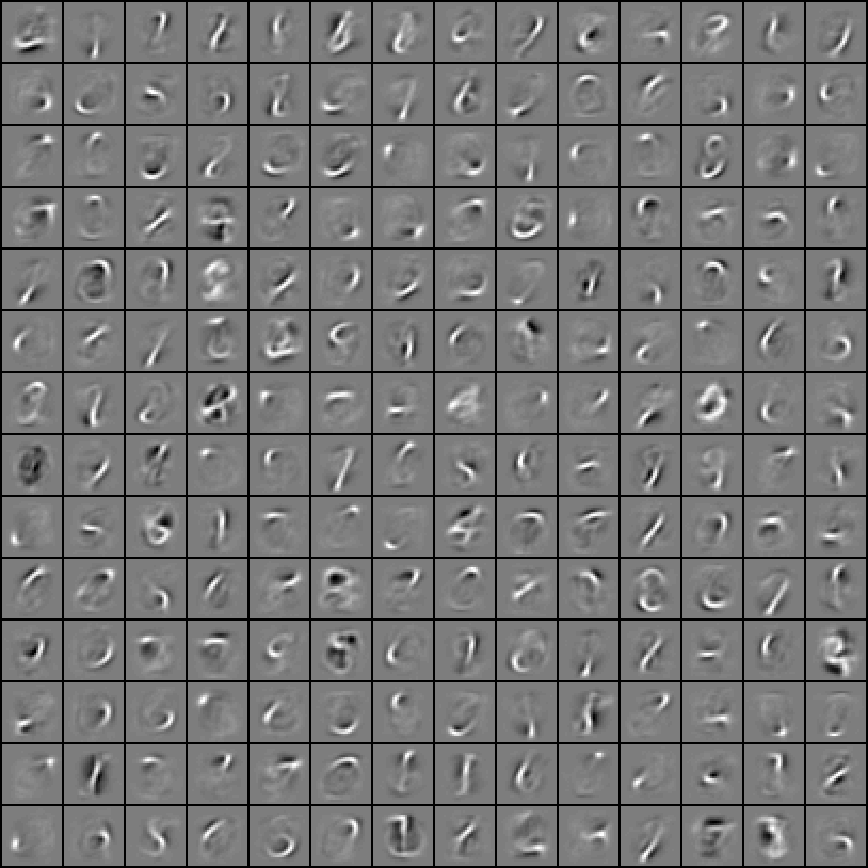
\includegraphics[width=0.6\textwidth]{figures/MnistVectorizationEx.png}
  %\caption{}\label{fig:step1}
\end{figure}

\cnt{If your parameters are improperly tuned, or if your implementation of the autoencoder is buggy, you may get one of the following images instead:}
    {}
    {}
\begin{figure}[ht] \centering
  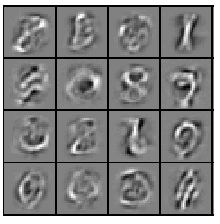
\includegraphics[width=0.4\textwidth]{figures/MNIST-false-bad-1.png}
  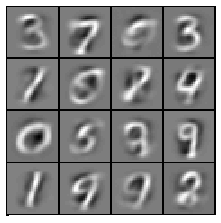
\includegraphics[width=0.4\textwidth]{figures/MNIST-false-bad-2.png}
  %\caption{}\label{fig:step1}
\end{figure}


\subsection{\cnt{Backpropagation vectorization hints}{反向传播矢量化提示}{}} \label{chp:backpropvechints}

Here, we give a few hints on how to vectorize the Backpropagation step. The hints here specifically build on our earlier description of how to vectorize a neural network(\ref{chp:neuralnetvec}).

Assume we have already implemented the vectorized forward propagation steps, so that the matrix-valued \texttt{z2, a2, z3} and \texttt{h} have already been computed. Here was our unvectorized implementation of \texttt{backprop}:
\begin{lstlisting}[language=matlab]
gradW1 = zeros(size(W1));
gradW2 = zeros(size(W2)); 
for i=1:m,
  delta3 = -(y(:,i) - h(:,i)) .* fprime(z3(:,i)); 
  delta2 = W2'*delta3(:,i) .* fprime(z2(:,i));
 
  gradW2 = gradW2 + delta3*a2(:,i)';
  gradW1 = gradW1 + delta2*a1(:,i)'; 
end;
\end{lstlisting}

Assume that we have implemented a version of \texttt{fprime(z)} that accepts matrix-valued inputs. We will use matrix-valued \texttt{delta3, delta2}. Here, \texttt{delta3} and \texttt{delta2} will have m columns, with one column per training example. We want to compute \texttt{delta3, delta2, gradW2} and \texttt{gradW1}.

Consider the computation for the matrix \texttt{delta3}, which can now be written:
\begin{lstlisting}[language=matlab]
for i=1:m, 
  delta3(:,i) = -(y(:,i) - h(:,i)) .* fprime(z3(:,i)); 
end;
\end{lstlisting}

Each iteration of the for loop computes one column of \texttt{delta3}. You should be able to find a single line of Matlab to compute \texttt{delta3} as a function of the matrices \texttt{y, h} and \texttt{z3}. This lets you compute \texttt{delta3}. Similarly, you should also be able to find a single line of code to compute the entire matrix \texttt{delta2}, as a function of \texttt{W2, delta3} (which is now a matrix), and \texttt{z2}.

Next, consider the computation for \texttt{gradW2}. We can now write this as:
\begin{lstlisting}[language=matlab]
gradW2 = zeros(size(W2));
for i=1:m, 
  gradW2 = gradW2 + delta3(:,i)*a2(:,i)';
end;
\end{lstlisting}

You should be able to find a single line of Matlab that replaces this for loop, and computes \texttt{gradW2} as a function of the matrices \texttt{delta3} and \texttt{a2}. If you're having trouble, take another look at the Logistic Regression Vectorization Example(\ref{chp:logisticvecexample}), which uses a related (but slightly different) vectorization step to get to the final implementation. Using a similar method, you will also be able to compute \texttt{gradW1} with a single line of code.

When you complete the derivation, you should be able to replace the unvectorized backpropagation code example above with just 4 lines of Matlab/Octave code. 
